\capitulo{5}{Aspectos relevantes del desarrollo del proyecto}

Este capítulo pretende recoger los aspectos más destacados y las decisiones de diseño adoptadas durante el ciclo de vida de SugAIr. En lugar de realizar una descripción exhaustiva del código fuente, se documentan los caminos de solución elegidos ante los retos técnicos planteados, con especial énfasis en la arquitectura del sistema, el ciclo de trabajo ágil y la integración del modelo de Inteligencia Artificial local.



\section{Inicio del proyecto y metodología de trabajo}
El origen del proyecto surge de la colaboración entre la Universidad de Burgos y el Programa Observatorio Tecnológico HP SCDS. A partir de los requisitos iniciales, se estableció un flujo de trabajo ágil apoyado en la plataforma GitLab, lo que permitió abandonar el desarrollo no estructurado en favor de un control iterativo basado en entregas de valor.

El progreso se dividió en ciclos de trabajo (sprints) gestionados mediante un tablero Kanban, garantizando la trazabilidad de cada tarea (\textit{issue}). A nivel organizativo, las primeras fases del desarrollo se estructuraron de la siguiente manera:

\begin{itemize}
    \item \textbf{Sprint 1: Preparación del entorno.} Dedicado a la instalación y configuración de las herramientas base del ecosistema, incluyendo VSCode, el entorno de React Native y el compilador de Go.
    \item \textbf{Sprint 2: Pruebas de concepto y esqueleto.} Generación de los primeros \textit{endpoints} de validación (healthcheck) en el servidor y creación del proyecto base en el frontend para establecer la comunicación inicial.
    \item \textbf{Sprint 3: Despliegue de IA local.} Fase de investigación orientada a la descarga de Ollama y la búsqueda de modelos de lenguaje compatibles con las especificaciones de hardware del equipo de desarrollo.
    \item \textbf{Sprint 4: Integración y control de la IA.} Establecimiento de las peticiones HTTP desde el servidor Go hacia Ollama, creación de la interfaz de chat en React y aplicación de ingeniería de \textit{prompts} para restringir las respuestas del modelo.
    \item \textbf{Sprint 5: Modelo multimodal, documentación y cierre.} Investigaición e implementación de un modelo multimodal y adaptación de la UI para adjuntar imágenes.
    Tambien acabar la documentación.
\end{itemize}
\clearpage
\begin{figure}
    \centering
    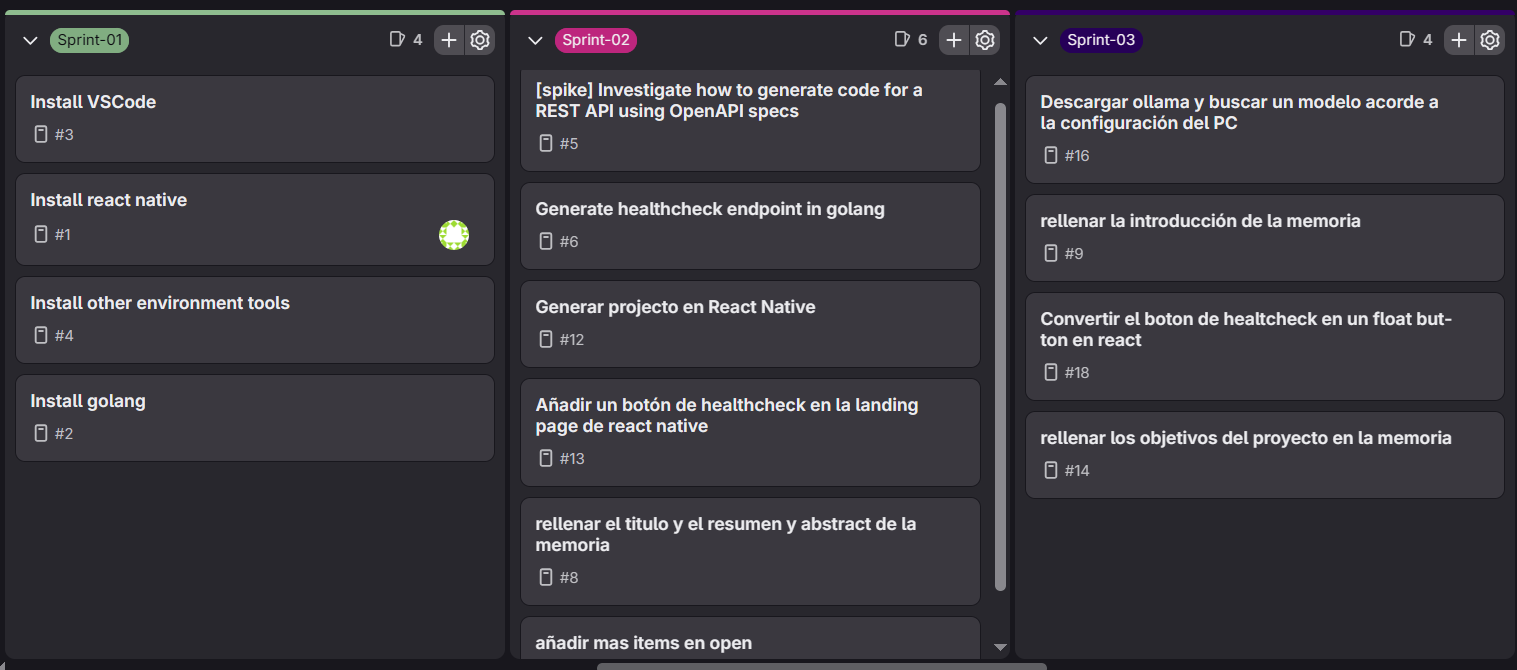
\includegraphics[width=0.75\linewidth]{tablero1.png}
    \caption{Sprints 1-3 en el tablero kanban}
    \label{fig:tablero1}
\end{figure}

\begin{figure}
    \centering
    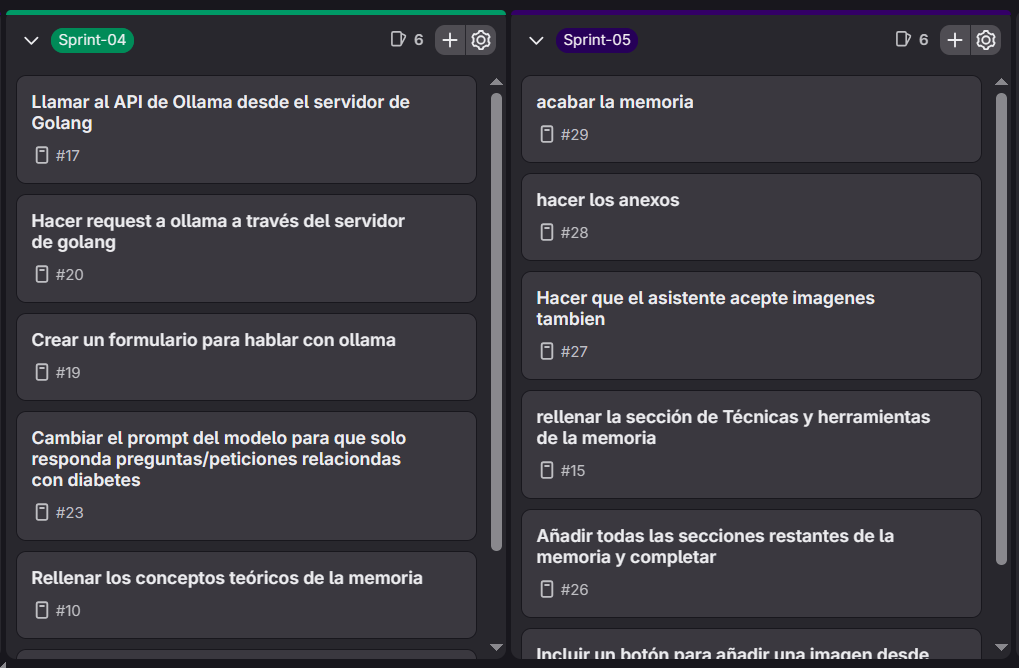
\includegraphics[width=0.75\linewidth]{tablero2.png}
    \caption{sprints 4-5}
    \label{fig:tablero2}
\end{figure}
\clearpage

\section{Desarrollo y arquitectura del backend}
El núcleo de la lógica de negocio y la gestión de peticiones reside en un servidor backend desarrollado en Go. Su función principal es actuar como una capa de seguridad y orquestación.

Para la comunicación con el motor de Inteligencia Artificial, se descartó la implementación de integraciones complejas basadas en librerías de terceros, optando por una solución más limpia y mantenible: el uso de peticiones HTTP directas contra la API REST que expone Ollama en el entorno local (localhost). Este diseño convierte al servidor en Go en un intermediario (proxy) que recibe los datos del frontend, lo formatea adecuadamente inyectando las directrices del sistema, y lo envía al modelo. 

Esta arquitectura presenta una ventaja crítica: si en el futuro se decide migrar de Ollama a otro entorno de ejecución local (como vLLM o llama.cpp), la aplicación cliente no sufrirá ningún impacto, ya que la adaptación se realizará de forma transparente y centralizada en el servidor Go.

\section{El problema de la ejecución local y las restricciones de hardware}
La integración de Modelos de Lenguaje Grande (LLM) supuso el mayor desafío técnico del proyecto. El objetivo inicial contemplaba el uso del modelo Llama 3.2 en su variante multimodal, con el fin de procesar tanto las consultas textuales del usuario como imágenes adjuntas (por ejemplo, gráficas de glucosa o etiquetas de alimentos).


Sin embargo, durante la fase de análisis (\textit{Sprint} 3), se evidenció un cuello de botella crítico: los requerimientos para la carga de un modelo base con capacidades de visión artificial excedían la memoria RAM disponible en el entorno de ejecución inicial. 

Para solventar esta limitación técnica sin comprometer el requisito fundamental de privacidad y ejecución local, se analizó el ecosistema de modelos optimizados, optando finalmente por la implementación de \textbf{Llava} (\textit{Large Language and Vision Assistant}) gestionado a través del motor Ollama. La viabilidad de esta integración radica en las técnicas de cuantización de pesos neuronales que emplea dicha plataforma, las cuales reducen drásticamente la huella en memoria del modelo permitiendo su despliegue en \textit{hardware} de consumo estándar sin una pérdida significativa de capacidad deductiva.

La elección de Llava se fundamenta en su arquitectura de vanguardia, la cual integra un codificador visual basado en la tecnología CLIP con el potente modelo de lenguaje LLaMA. Esta fusión permite al sistema interpretar de manera conjunta instrucciones semánticas y matrices de píxeles, resultando idóneo para la lectura y compresión de etiquetas nutricionales complejas.

Para adaptar esta herramienta al contexto médico del proyecto, se desarrolló una variante específica denominada \texttt{llava-diabetes}. A través de la configuración de un archivo nativo (\textit{Modelfile}), se empaquetó el modelo base cuantizado junto con un mapa de directrices (\textit{system prompt}). Este contexto preinyectado restringe el ámbito de actuación del asistente, asegura un tono profesional e impersonal, y estandariza la extracción de macronutrientes, superando así las restricciones de \textit{hardware} iniciales y consolidando un flujo multimodal robusto.

Adicionalmente, para dotar al modelo de utilidad clínica real, se aplicaron técnicas de ingeniería de contexto (\textit{prompt engineering}). Se configuró el comportamiento base del modelo para que actúe estrictamente como un educador diabetológico, programándolo para rechazar de forma controlada y segura cualquier consulta o interacción que no esté directamente relacionada con la diabetes.

\section{Desarrollo del frontend}
La capa de presentación se implementó mediante React, configurado para ejecutarse en un entorno web simulando una disposición móvil.

La interfaz principal consta de una aplicación de página única (\textit{Single Page Application}) que emula el comportamiento de plataformas de mensajería instantánea. Se han utilizado componentes dinámicos para el renderizado de chat, la entrada de texto y el manejo de los estados de carga (\textit{loading states}) mientras el servidor aguarda la inferencia generada por la Inteligencia Artificial.

\begin{figure}
    \centering
    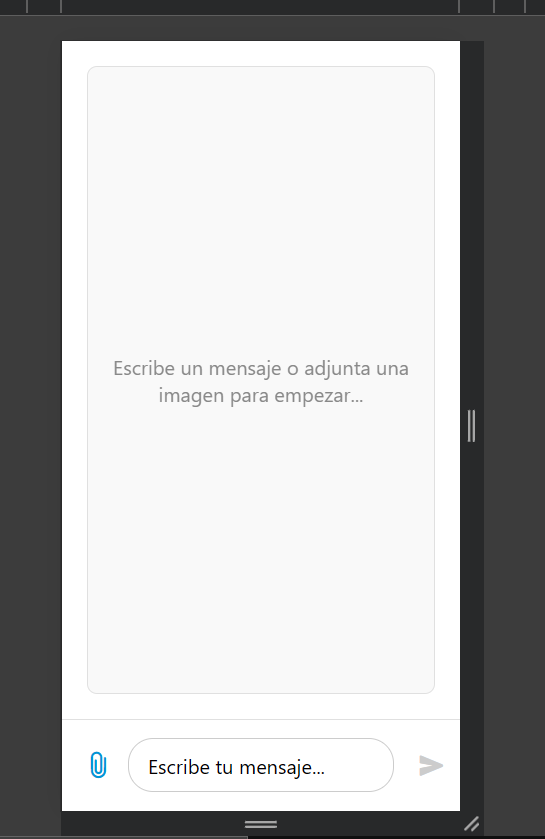
\includegraphics[width=0.75\linewidth]{frontend.png}
    \caption{pantalla inicial de la interfaz gráfica}
    \label{fig:placeholder}
\end{figure}